\chapter{\;\;\;\;Verification Techniques}
\label{sec:overview-verification}

We review the notions of closed and open simulations
(\Cref{sec:overview-verification:background}), discuss the problems
with open simulations
(\Cref{sec:overview-verification:problems}) and present our solution
(\Cref{sec:overview-verification:solution}).
We also discuss the memory relations used by \ccm{} in \Cref{sec:overview-verification:injection}
and present mixed simulations in \Cref{sec:overview-verification:mixedsim}.

\section{Background}
\label{sec:overview-verification:background}

\myparagraph{\cc{}'s Verification}

\cc{}'s correctness establishes \emph{behavioral refinement}
(also called \emph{semantics preservation}) saying that
the set of all observable behaviors of a source program~$P$, denoted $\beh{P}$ (seen as a specification),
includes that of its compiled target program~$Q$, \ie $\beh{Q}$ (seen as an implementation).
Here an observable behavior of a program (either in C, assembly, or an
intermediate language) is a (finite or infinite) trace of observable events
(typically, invocation of system calls) occurring in a sequence of execution steps according to the language semantics.

The semantics of a language $\mathbb{L}$ is given by a loading
function ${\load} \in \Prgs{\mathbb{L}} \to \Memory\times\States{\mathbb{L}}$
from programs to \emph{machine states} consisting of a memory and a \emph{language state},
and a step relation
${\step} \subseteq { (\Memory\times\States{\mathbb{L}}) \times \Events \times (\Memory\times\States{\mathbb{L}})}$
between machine states producing an event.
Specifically, $\load{P}$ denotes the initial machine state after loading the program $P$, and
$(\mem,\stt) \estep{e} (\mem',\stt')$ denotes that the machine state $(\mem,\stt)$ can transition to
$(\mem',\stt')$ producing an (observable or silent) event $e$ in a single step of
execution.
%% Finally, a behavior of program $P$ is a (finite or
%% infinite) sequence of observable events that appear in a sequence of
%% execution steps from the initial state of $P$.

\cc{} is a multi-pass compiler and the whole verification is performed modularly
by composing independent verification of each pass. Specifically,
verification of a pass proves that the source and target programs of every translation
performed by the pass are related by a certain relation,
called (closed) \emph{simulation}, to be described below.
Since simulation relations are closed under composition, every
end-to-end translation, which is a composition of translations of all
passes, is also related by a simulation relation. Finally, \cc{}'s
correctness follows from the fact that every simulation relation implies
behavioral refinement between the related programs.

In fact, there are two versions of simulations, \emph{forward}
and \emph{backward}.  The former is more convenient for compiler
verification but implies behavioral refinement only when the target
language is deterministic\footnote{\cc{} uses a slightly different
  condition, namely that the source language is \emph{receptive} and
  the target is \emph{determinate}.}. Since \cc{} mostly uses forward
simulations, we will also focus on forward ones throughout the paper
and discuss how to mix forward and backward simulations
to support forward reasoning even when the target language is not deterministic
in \Cref{sec:overview-verification:mixedsim}.

%% Though there are two dual notions of simulations, \emph{forward} and
%% \emph{backward}, and \cc{} mostly uses forward simulations, here we
%% focus on forward simulations for simplicity and will discuss both
%% simulations in details in \Cref{sec:overview-verification:mixedsim}.
%% \todo{========= Turn backward into forward ===========}

We say a translation of a program $P$ into $Q$ is related by a
relation $R$ between machine states if the loaded initial states
$\load{P}$ and $\load{Q}$ are related by $R$.
Then $R$ is called a (closed forward) simulation if for any
pair of machine states $(\mssrc,\mstgt)$ related by $R$, the target state $\mstgt$ simulates one step
execution of the source state $\mssrc$ (up to silent steps, denoted $\tau$) and the resulting
states are again related by $R$ (slightly simplified for presentation purposes):
\[
\begin{array}{r@{\ \ }l}
  \forall (\mssrc, \mstgt) \in R,~ \forall e, \mssrc',~&
  \mssrc \estep{e} \mssrc' \implies {}\\[1mm]
  \exists \mstgt',~&
  \mstgt \estep{\tau}^{\raisebox{-1mm}{\scriptsize$\ast$}} \estep{e}\estep{\tau}^{\raisebox{-1mm}{\scriptsize$\ast$}} \mstgt' \land (\mssrc', \mstgt') \in R~.
\end{array}
\]
%% By repeating this simulation step, one can easily see that $\beh{P} \supseteq \beh{Q}$ holds.
%% Also, it is not hard
%% to see that such simulation relations are closed under composition.
%% \jeehoon{Should we say it's a little bit simplified version?  E.g. we're omitting stuttering here.}

\myparagraph{\ccc{}'s Verification}

% \emph{core semantics}
The interaction semantics of \ccc{} gives a way to execute an
\emph{open} module $\module$ (\ie invoking external functions defined
outside $\module$) in isolation by providing a logical mechanism to
reflect possible interference from external function calls. More
specifically, the semantics provides two meta-level functions
$\mathtt{at\_external}$ and $\mathtt{after\_external}$. First,
$\mathtt{at\_external}~\stt = \mathtt{Some}~(f,\vec{v})$ denotes that
at language state $\stt$, an external function pointed to by a
function pointer $f$ is called with arguments $\vec{v}$. Second,
$\mathtt{after\_external}~r~\stt$ denotes the language state after the
external function call at $\stt$, assuming the call returned a value
$r$.
%% See \Cref{sec:overview-semantics:background} and \Cref{sec:main-semantics}
%% for more details about the interaction semantics.

%% $\mathtt{at\_external}$ detecting an external function call:
%% $\mathtt{at\_external}~\stt = \mathtt{Some}~(f,\vec{v})$ denotes that
%% at language state $\stt$, an external function pointed to by a
%% function pointer $f$ is called with arguments $\vec{v}$. Also, it
%% provides a meta-level function $\mathtt{after\_external}$ constructing the language state after
%% an external function call: $\mathtt{after\_external}~r~\stt$ denotes
%% the language state after the external function call at $\stt$, assuming
%% the call returned a value $r$. See \Cref{sec:main-semantics} for more details
%% about the interaction semantics.
%% \jeehoon{I don't think it's necessary to mention the word ``core semantics''. Why not just saying
%%   it's interaction semantics?}

Using interaction semantics, \ccc{} defines \emph{structured
  simulations} relating two open modules.
Here we briefly review the key ideas behind them,
which also occurred elsewhere, \eg in~\cite{pb,neis:pilsner,PLDI15}. \todo{check PLDI15}
First, unlike the closed simulations above,
structured simulations explicitly specify value and memory relations
(evolving over time) because values and memory are shared with external modules.
Specifically, such relations are defined using Kripke-style possible worlds,
called \emph{structured injections} \revision{(see \Cref{sec:overview-verification:injection} for more details)},
by giving $(i)$ a future world relation $\sqsupseteq$ for which
$w' \sqsupseteq w$ denotes that $w'$ is a future world of $w$;
and $(ii)$ value and memory relations at each world~$w$, denoted
$\mathtt{vrel}(w)$ and $\mathtt{mrel}(w)$.  Then, a
structured simulation $R$ gives a relation between machine
states at each world $w$, denoted $R(w)$, and should satisfy the
\emph{open} simulation property (simplified for presentation purposes) given in \Cref{fig:open-sim}.
\begin{figure}[t]
$
\begin{array}{@{}l@{}}
\texttt{ 1:}~\forall w,~ \forall (\memsrc,\memtgt)\in \mathtt{mrel}(w),~\forall \stsrc,\sttgt,~((\memsrc,\stsrc),(\memtgt,\sttgt))\in R(w)\implies{} \\[.5mm]
\texttt{ 2:}~\quad\textbf{match}~\mathtt{at\_external}~\stsrc~\textbf{with}\\[.5mm]
\texttt{ 3:}~\quad\mathtt{|}~\mathtt{Some}~(f_\src,\vec{v}_\src) \Rightarrow{}\\[1mm]
\texttt{ 4:}~\quad\quad \exists f_\tgt,\vec{v}_\tgt,~ \mathtt{at\_external}~\sttgt = \mathtt{Some}~(f_\tgt,\vec{v}_\tgt) \land{}\\[1mm]
\texttt{ 5:}~\quad\quad \fbox{$(f_\src,f_\tgt)\in \texttt{vrel}(w) \land (\vec{v}_\src,\vec{v}_\tgt) \in \overrightarrow{\texttt{vrel}(w)}$} \land{} \\[2mm]
\texttt{ 6:}~\quad\quad \dashbox{$\forall w' \sqsupseteq w,~\forall (\memsrc',\memtgt')\in\texttt{mrel}(w')$,}~ \dashbox{$\forall (r_\src,r_\tgt)\in \texttt{vrel}(w'),$}\\[2.5mm]
\texttt{ 7:}~\quad\quad ((\memsrc',\mathtt{after\_external}~r_\src~\stsrc),(\memtgt',\mathtt{after\_external}~r_\tgt~\sttgt))\in R(w') \\[.5mm]
\texttt{ 8:}~\quad\mathtt{|}~\mathtt{None} \Rightarrow{} \\[-.5mm]
\texttt{ 9:}~\quad\quad\forall e, \memsrc', \stsrc',~ (\memsrc, \stsrc) \estep{e} (\memsrc',\stsrc') \implies {}\\[.5mm]
\texttt{10:}~\quad\quad \exists \memtgt',\sttgt',~ (\memtgt,\sttgt) \estep{\tau}^{\raisebox{-1mm}{\scriptsize$\ast$}} \estep{e}\estep{\tau}^{\raisebox{-1mm}{\scriptsize$\ast$}} (\memtgt',\sttgt') \land{}\\[1mm]
\texttt{11:}~\quad\quad \fbox{$\exists w' \sqsupseteq w,~ (\memsrc',\memtgt') \in \mathrm{mrel}(w')$} \land {} \\[2.5mm]
\texttt{12:}~\quad\quad((\memsrc',\stsrc'), (\memtgt',\sttgt')) \in R(w')\\
\texttt{13:}~\quad\textbf{end}
\end{array}
$
\caption{Structured (or, open) simulations (simplified for presentation purposes)}
\label{fig:open-sim}
\end{figure}
% \jeehoon{In \texttt{at\_external} case, how about allowing the source to take silent steps?  Or
%   maybe we can remove silent steps also from the previous paragraph on CompCert's verification.}

Here the simulation involves rely-guarantee reasoning and is split
into two cases: one for interactions with external modules and the
other for internal steps (omitting two more cases for function start and end,
for presentation purposes). Specifically, given
any world $w$, related memories at $w$ and machine states related by
the simulation relation $R$ at $w$ (line~1), we check whether the
source state is invoking an external function or taking an internal
step (line~2). In the former case (line~3), the target state should
also be invoking an external function (line~4) and the invoked
functions and arguments should be related by the value relation at the
world~$w$ (line~5), which is a \fbox{guarantee condition} to the external modules.
Then we assume that the invoked external
functions proceed to a future world $w'$ yielding related memories and
related return values at $w'$ (line~6), which is a \dashbox{rely condition} from the external modules.
Under the assumption, the machine
states after the external calls should also be related by the
simulation relation $R$ at the future world $w'$ (line~7). In the
latter case (line~8), for any internal step from the source state
(line~9), there should be corresponding internal steps from the
target state (line~10).  Then the resulting memories after the steps
should be related at some future world $w'$ (line~11), which is a
\fbox{guarantee condition} to the external modules.  Finally, the
machine states after the steps should also be related by the
simulation relation $R$ at the future world $w'$ (line~12).

At high level, this simulation property specifies that internal
executions of the source and target modules should be related in
lockstep satisfying the guarantee conditions to the external modules,
assuming that the rely conditions from them hold after each external
function call.  Note that the rely and guarantee conditions on memory
(at lines 6 and 11) are matched and also those on values (at lines 5
and 6) will be matched if we include the omitted cases for function
start and end. This matching---in addition to the fact that the same
rely/guarantee conditions are used globally (\ie for verification of
every module)---is crucial for proving preservation of the simulation
property after linking modules because otherwise what one module
assumes about the other modules will not match with what the other
modules guarantee.

To use structured simulations for compiler verification, \ccc{} proves
the following three key properties, where we say a source module
$\module$ simulates a target module $\module'$ if there exists a
structured simulation that relates $\module$ and $\module'$:
\begin{itemize}
\item \textbf{(\emph{Vertical Compositionality})}
  If $\module$ simulates $\module'$, which simulates $\module''$,
  then $\module$ simulates~$\module''$.
\item \textbf{(\emph{Horizontal Compositionality})}
  If $\module_1$ and $\module_2$ simulate
     $\module'_1$ and $\module'_2$ respectively,
  then the linked source module  $\module_1 \llink \module_2$ simulates
  the linked target module $\module'_1 \llink \module'_2$.
\item \textbf{(\emph{Adequacy})}
  If $\module$ simulates $\module'$,
  then $\beh{\module} \supseteq \beh{\module'}$.
\end{itemize}

\section{Problems}
\label{sec:overview-verification:problems}
%% \myparagraph{Problems}
%
%   9051 /   2839 = 3.2 (id)
%  22124 /   8129 = 2.7 (ext)
%  23564 /   9128 = 2.6 (inj)
%
% Total
%  54739 /  20096 = 2.7  (pass)
% 152363 /  92029 = 1.65 (meta)
% 207102 / 112125 = 1.84 (whole)
%
%% Structured simulations of \ccc{} suffer from the problem that
%% verification using them is significantly more costly than that using
%% closed simulations of \cc{}: the Coq scripts for the verification of
%% all passes in \ccc{} is roughly \todo{2.7} times as large as that in
%% the original \cc{} in terms of lines of code~(LOC).
%% \jeehoon{How about reporting significant lines of code (SLOC)?}

As discussed in the introduction, verification using structured
simulations is significantly more costly than that using closed
simulations.  The reasons are twofold.

First, \revision{while closed simulations freely allow arbitrary memory relations---%
therefore \cc{} uses three different kinds of memory relations to simply proofs---%
%% ---thereby \cc{} uses three relations, \emph{memory identity, extension and injection}---
structured simulations only allow a single type of memory relations
called \emph{structured injections} due to horizontal compositionality.}
%
The reason is that, as discussed above,
%% in the background section,
allowing different memory relations would introduce
different rely/guarantee conditions
thereby breaking simulation after linking (\ie horizontal
compositionality) due to the mismatch between different rely/guarantee
conditions.
%% To see the reason, recall that, as we have seen in the
%% background section, the rely/guarantee conditions are determined by the
%% memory (and value) relations and the same rely/guarantee conditions
%% should be used globally to preserve simulations after linking
%% modules (\ie to prove horizontal compositionality).
%% Therefore allowing different memory relations for verifying
%% different modules would be problematic for proving horizontal
%% compositionality together with adequacy.

\revision{Second,
%% the notion of structured injection of \ccc{} is more complex than that of
%% \emph{memory injection} of \cc{} and, as far as we understand, such
%% complexity is needed for vertical compositionality.
%% It is well known that
proving vertical compositionality for \emph{open} simulations is in general
very technical and involved~\cite{ICFP19,neis:pilsner}. Indeed the
proof for structured simulations is about 5,000 SLOC in Coq.
Moreover, vertical compositionality also introduces unnecessary complexities
in structured simulations of \ccc{} such as \emph{effect annotations}
and \emph{closedness under restriction} \cite{stewart:ccc}.}
%% which makes correctness proofs of compiler passes more involved
%% (see \Cref{sec:overview-verification:injection} for discussion).}

To sum up, although it is quite straightforward to prove horizontal
compositionality and adequacy for a single relation (\ie with the same
rely/guarantee conditions), it is challenging to prove $(i)$ vertical
compositionality even for a single relation and $(ii)$ horizontal
compositionality between different relations (\ie with different
rely/guarantee conditions).

%\section{Refinement Under Self-related Contexts (RUSC)}
\section{Our Solution}
\label{sec:overview-verification:solution}

%% \myparagraph{Our Solution at High Level}
%
Our solution is twofold. First, we develop a general and abstract
theory, called \emph{Refinement Under Self-related Contexts (RUSC)},
which is inspired by the standard notion of contextual refinement
\revision{and the notion of self-related context from \cite{stewart:ccc}
  (see \Cref{sec:related} for comparison).}
%\scc{}~\cite{?} (see \Sref{sec:related} for comparison).
Specifically, given a set of (arbitrary and independent)
relations each of which is horizontally compositional and adequate,
RUSC completes the relations by giving a super-relation (\ie
including all of them) that is horizontally and vertically
compositional and also adequate. Second, we prove that
our version of structured simulations, called \emph{open simulations},
with almost arbitrary memory relations
are horizontally compositional and adequate,
so that we can apply RUSC to open simulations with any chosen set of memory relations.

\myparagraph{Theory of RUSC}
%
RUSC can be defined abstractly for any linking algebra, which consists
of a set of modules, $\Module$, with a notion of behavior\footnote{Behaviors just need to be defined for closed programs.
  Technically, we can give undefined behavior (UB) to open modules.
%  For open modules, invoking an unknown function can be defined as undefined behavior (UB).
}, denoted
$\beh{p}$ for $p\in\Module$, a linking operation~$\llink$ between modules
that is associative%
\footnote{\revision{Commutativity does not hold for linking of \cc{} modules
    because changes in the order of global variables affect the initial memory after loading
    due to \cc{}'s deterministic memory allocation.}},
\revision{and the identity (\ie empty) module $\identity \in \Module$}:
\[
\begin{array}{c}
\llink: \Module \times \Module \rightarrow \Module \\
\forall p,q,r\in\Module,~p \llink (q \llink r) = (p \llink q) \llink r \\
\revision{\forall p \in\Module,~ \identity \llink p = p \llink \identity = p} \\
\end{array}
\]
Note that RUSC can be applied to interaction semantics because it
allows linking between arbitrary modules sharing the same notions
of value and memory (see \Cref{sec:overview-semantics:background} and \Cref{sec:main-semantics} for details).

To define RUSC, let $\rels$ be a set of module relations each of which is horizontally
compositional and adequate: for any $R \in \rels$ and $p,p',q,q'\in \Module$,
\[
\begin{array}{r@{}l@{\qquad}l}
(p,p'),(q,q')\in R &{}\implies (p \llink q, p' \llink q') \in R &\textrm{(\emph{HorComp})} \\
(p,p') \in R &{}\implies \beh{p} \supseteq \beh{p'} &\textrm{(\emph{Adequacy})} \\
\end{array}
\]
Then the RUSC relation for $\rels$, denoted $\rusc_{\rels}$, is defined as follows:
\[
\begin{array}{rcl}
p \rusc_{\rels} p' &\text{\emph{iff}}& \revision{\forall c_1, c_2 \in \self{\rels},~
\beh{c_{1} \llink p  \llink c_2} \supseteq \beh{c_{1} \llink p' \llink c_2}} \\
\self{\rels} & \defeq & \setof{ c \in \Module \suchthat \forall R \in \rels,~ (c,c) \in R }
\end{array}
\]
The definition is simple: $p$ is RUSC-related to $p'$ if the behaviors of $p'$ refine those of $p$ under
arbitrary contexts that are related to themselves by every relation in $\rels$.
% \jeehoon{From the definition of $p \rusc_{\rels} p'$, I think maybe it's easier to distinguish the
%   module type and the list-of-modules type... I know it's vague. Let's discuss offline.}

\begin{theorem}[Properties of RUSC]\label{thm:rusc} The RUSC relation $\rusc_\rels$ satisfies the following key properties.\\[.5mm]
$
\begin{array}{@{\quad}lrl}
 \text{(Inclusion)} &\forall R \in \rels,& R \subseteq {\rusc_\rels} \\[.5mm]
 \text{(Adequacy)} &\forall p,p'\in\Module,& p \rusc_{\rels} p' \implies \beh{p} \supseteq \beh{p'} \\[.5mm]
 \text{(VerComp)} &\forall p,p',p''\in\Module,& p \rusc_{\rels} p' \land p' \rusc_{\rels} p'' \implies p \rusc_{\rels} p'' \\[.5mm]
 \text{(HorComp)} &\forall p,p',q,q'\in \self{\rels},&   p \rusc_{\rels} p' \land  q \rusc_{\rels} q' \implies p \llink q \rusc_{\rels} p' \llink q' \\[.5mm]
 \revision{\text{(SelfComp)}} & \revision{\forall p,q \in \self{\rels},}& \revision{p \llink q \in \self{\rels}}
\end{array}
$
\end{theorem}
Note that horizontal compositionality holds only for self-related
modules, which, however, is not a big deal in practice as we will
discuss below.
\begin{proof}
The proof of the theorem is simple.  The
inclusion $R \subseteq {\rusc_\rels}$ trivially follows from the
horizontal compositionality and adequacy of $R$.  Adequacy of
$\rusc_\rels$ directly follows from the definition of $\rusc_\rels$ by
taking the empty context. Vertical compositionality (\ie transitivity)
of $\rusc_\rels$ holds trivially by definition.  Horizontal
compositionality, $p \llink q \rusc_{\rels} p' \llink q'$, is proven
in two steps using transitivity: $(i)$ $p \llink q \rusc_{\rels} p' \llink q$,
which follows from the definition of $p \rusc_{\rels} p'$ since $q\in\self{\rels}$,
and $(ii)$ $p' \llink q \rusc_{\rels} p' \llink q'$, which follows
similarly since $q \rusc_{\rels} q'$ and $p'\in\self{\rels}$.
%% ${R} \subseteq {\rusc_{\setofz{R}}}$ and
%% ${\rels} \subseteq {\rels'} \implies {\rusc_{\rels}} \subseteq {\rusc_{\rels'}}$
\revision{Finally, self-relatedness is closed under composition
because every relation in $\rels$ is horizontally compositional.}
\end{proof}

The reason why vertical compositionality is easily proven for RUSC
is that we essentially prove it for \emph{closed} programs by
closing an open module with contexts. Indeed, the technical
difficulties with vertical compositionality for open
simulations arise from the openness: it is difficult to set up a
setting properly with arbitrary future memories given after an external
function call.

The reason why horizontal compositionality holds between different
relations is interesting. Directly composing two simulations $(p,p') \in R_1$
and $(q,q') \in R_2$ with different relations $R_1$ and $R_2$
does not work in general. However, each simulation can be easily
extended with identical contexts because a pair of identical modules
usually respects any sensible relational principles. Therefore,
we have $(p \llink q ,p' \llink q) \in R_1$ and
$(p' \llink q ,p' \llink q') \in R_2$, which can be transitively composed
by vertical compositionality just as discussed above.
%% \jeehoon{I think we can say our horizontal compositionality proof, not the entire RUSC, is inspired
%%   from \scc{}.}

To sum up, RUSC provides a general condition for composing
different relational proofs: each proof just needs to be compatible
with its context modules in terms of self-relatedness, not necessarily
with their relational proofs.
%% instead of their relational proofs.

%% \begin{figure}
%%   \centering
%%   \includegraphics[width=0.70\linewidth]{rusc.jpg}
%%   \caption{Proving compositional compiler correctness with RUSC
%%   }
%%   \label{fig:rusc}
%% \end{figure}

%% \todo{add a fig:
%%   small horizontal compositionality figure,
%%   say that compatibility of rely/guarantee conditions between two relations (no)
%%   say that compatibility of rely/guarantee condition vs. the context I linked with. (yes)
%% }

\myparagraph{Open Simulations}
%
%% \todo{talk about analysis}
%% Since we can obtain vertical and horizontal compositionality
%% using RUSC, we can use simpler simulation relations (with different
%% memory relations)---which we call \emph{open simulations}---than
%% structured simulations (with structured injections).
%% Basically, open simulations contain only the core mechanism of
%% structured simulation presented in \Cref{sec:overview-verification:background}
%% without unnecessary complications needed to prove vertical
%% compositionality.

\revision{Since we can obtain vertical and horizontal compositionality using RUSC,
we can use open simulations with almost arbitrary memory relations.}
More specifically, we prove that open simulations with
\emph{any} Kripke-style memory/value relation satisfying certain minimal
conditions (see \Cref{sec:main-verification:parameter} for details) are horizontally compositional
and adequate. Since the required conditions are so minimal, they are
satisfied by the three memory relations---memory identity, extension
and injection---and also by a more powerful relation,
called \emph{memory injection with module-local invariants}.
This new memory relation is needed to
verify a new pass we added, called \texttt{Unreadglob}, which
requires reasoning about module-local states enabled by \emph{static}
variables of C (see \Cref{sec:overview-modulelocal} for details).

%% (emphasize that RUSC allows different techniques for different passes.
%% Additionally, analysis passes and assumptions on global variables).
Note that unlike \cc{} 2.1 on which \ccc{} is based, \cc{} 3.5
implements a static analyzer performing value analysis, which is used by
several passes. In order to support independent modular verification of such analyzers,
we also parameterize open simulations with memory predicates---representing the
analysis results of such analyzers---and
prove their horizontal compositionality and adequacy (See \Cref{sec:main-verification} for details).

\myparagraph{Applications} In our paper, we use RUSC
% with open simulations
in two situations: compiler and program verification.
%% \jeehoon{On paragraph name: how about ``Applications''?  It sounds more general.}

First, we give an abstract example for compiler
verification.  Suppose our source program is written in three modules,
\texttt{a.c}, \texttt{b.c} and \texttt{c.asm}, and compiled via
multiple passes: $\texttt{a.c}\to\texttt{a.il1}\to\texttt{a.asm}$ and
$\texttt{b.c}\to\texttt{b.il2}\to\texttt{b.il3}\to\texttt{b.asm}$,
each of which is verified using a different relation as follows:
\[
\begin{array}{l}
  (\texttt{a.c},\texttt{a.il1}) \in R_1 \quad (\texttt{a.il1},\texttt{a.asm}) \in R_2 \\
  (\texttt{b.c},\texttt{b.il2}) \in R_3 \quad
  (\texttt{b.il2},\texttt{b.il3}) \in R_4 \quad
  (\texttt{b.il3},\texttt{b.asm}) \in R_5
\end{array}
\]
%
Then as long as the \emph{end modules}, \texttt{a.c}, \texttt{b.c}, \texttt{a.asm},
\texttt{b.asm}, \texttt{c.asm}, are self-related by the relations $R_1,\ldots,R_5$,
using RUSC we can obtain the following behavioral refinement:
\[
\beh{\texttt{a.c} \llink \texttt{b.c} \llink \texttt{c.asm}} \supseteq \beh{\texttt{a.asm} \llink \texttt{b.asm} \llink \texttt{c.asm}}
\]
The underlying reasoning is simple: for $\rels=\setof{R_1,\ldots,R_5}$, we get
\begin{itemize}
\item $\texttt{a.c} \rusc_\rels \texttt{a.asm}$ and $\texttt{b.c} \rusc_\rels \texttt{b.asm}$
  by Inclusion and VerComp of \Cref{thm:rusc};
\item $\texttt{c.asm} \rusc_\rels \texttt{c.asm}$ since
  %% $\texttt{c.asm} \in \self{\rels}$ and thus
  $(\texttt{c.asm},\texttt{c.asm}) \in R_1 \subseteq \rusc_\rels$
  by Inclusion of \Cref{thm:rusc};
  %% \jeehoon{I don't understand it..}
\item $\texttt{a.c} \llink \texttt{b.c} \llink \texttt{c.asm} \rusc_\rels \texttt{a.asm} \llink \texttt{b.asm} \llink \texttt{c.asm}$
  by HorComp of \Cref{thm:rusc};
\item $\beh{\texttt{a.c} \llink \texttt{b.c} \llink \texttt{c.asm}} \supseteq \beh{\texttt{a.asm} \llink \texttt{b.asm} \llink \texttt{c.asm}}$ by Adequacy of \Cref{thm:rusc}.
\end{itemize}
Note that we need to prove the self-relatedness only for the end
modules because we only link those, not the intermediate ones
like \texttt{a.il1}, \texttt{b.il2}, \texttt{c.il3}.
Moreover, proving self-relatedness by a relation is typically
straightforward as long as the relation is sensibly defined.  Indeed,
we could easily prove that \emph{all} Clight\footnote{Clight is taken
  as the source language in most verification projects using \cc{}
  such as VST~\cite{VST}, CertiKOS and even \ccc{}.
  However, we also prove behavioral refinement w.r.t. the C source language
  (see \Cref{sec:results}).
}
and assembly programs are
self-related by all the relations used by \ccm{}
(\ie open simulations with memory identity, extension,
and injection with or without module-local invariants).
%% \jeehoon{How about ``we could easily prove that \emph{all} C, Clight, ...''}

Second, we demonstrate, via small but interesting examples (see \Cref{sec:overview-modulelocal}),
% (see \Cref{sec:overview-modulelocal} and \Cref{sec:utod-verification}),
%% the possibility
that our framework can be used to verify program modules
against (open) mathematical specification modules, written in Coq's Gallina language.
In the above example, for instance, we can prove
\[
\begin{array}{c}
\texttt{a.spec} \rusc_\rels \texttt{a.c}\quad
\texttt{b.spec} \rusc_\rels \texttt{b.c}\quad
\texttt{c.spec} \rusc_\rels \texttt{c.asm}
\\
\texttt{abc.spec} \rusc_\rels \texttt{a.spec} \llink \texttt{b.spec} \llink \texttt{c.spec}
\end{array}
\]
and link them together with the compiler correctness results above to get
\[
\beh{\texttt{abc.spec}}
\supseteq %% \rusc_\rels
%% \texttt{a.spec} \llink \texttt{b.spec} \llink \texttt{c.spec}
%% \rusc_\rels
\beh{\texttt{a.asm} \llink \texttt{b.asm} \llink \texttt{c.asm}}
\]
as long as the mathematical specification modules \texttt{a.spec},
\texttt{b.spec}, \texttt{c.spec}, \texttt{abc.spec} are in $\self{\rels}$,
which is usually straightforward to prove.

\myparagraph{Comparison to Contextual Refinement}
%
As one can easily see, RUSC refines the standard notion of contextual
refinement: instead of quantifying over \emph{all} contexts, RUSC
quantifies over only \emph{self-related} contexts. The main difference
is that RUSC gives the notion of well-behaved context w.r.t. a given
set of program relations (\ie reasoning principles) in terms of
contexts self-related by them.  This is particularly useful when not
all contexts are well behaved.  For example, in the interaction
semantics allowing mathematical specification modules as above, one can
easily write a specification module that arbitrarily changes the whole
memory including other modules' private memory. Under the presence of
such ill-behaved contexts, the contextual refinement will end up being too
strong preventing any reasoning about private memory such as
functions' stack frames. On the other hand, RUSC w.r.t. a set of
sensible relations will rule out such bad contexts and give us a sensible (better) relation.
%% even in the presence of such ill-behaved contexts.

%% \todo{Revise:
%% To sum up, the theory of RUSC tells that different relational proofs
%% well compose as long as the contexts of your interest are self-related
%% by the proof techniques of your interest.
%% }

%% because RUSC quantifies over only well-behaved contexts (\ie self-related ones
%% w.r.t. the given set of relations).

%% \hide{
%% We first review \cc{}'s correctness statement and its verification
%% method (\Cef{sec:background:cc}), and then how \ccc{} extends \cc{}
%% to allow multi-language programs (\ie programs composed of modules written in
%% different languages including C, assembly and \cc{}'s intermediate languages) (\Cref{sec:background:ccc}).
%% %% \ccc{} generalizes them to handle interactions between modules written in different
%% %% languages (\Cref{sec:background:ccc}).
%% In addition, we review key semantic techniques used for verification of CompCert.
%% %% called undefined behavior and logical memory
%% (\Cref{sec:background:ub}).
%% }

% BEGIN REVISION
{\revisioncmd
\section{Memory Relations of \ccm{}}
\label{sec:overview-verification:injection}

\ccm{} uses the original memory identity and extension of \cc{}
(\Cref{sec:overview-verification:injection:original}) and mildly
strengthens the original memory injection to reason about dynamically allocated
local memory such as a function's stack frame for \emph{open} modules,
which can be compared to the structured injection of \ccc{}
(\Cref{sec:overview-verification:injection:dynamic}).
Moreover, we generalize it further to reason about statically allocated local memory
such as static variables of C by allowing module-local invariants on those static variables
(\Cref{sec:overview-verification:injection:static}).

%% and mildly generalize the memory injection of \cc{} in two steps: first to reason
%% about dynamic local memory such as a function's stack frame
%% (\Cref{sec:overview-verification:injection:dynamic}) and further to
%% reason about static local memory such as static variables of C
%% (\Cref{sec:overview-verification:injection:static}).
%% Structured injections of \ccc{} can be compared to our first generalization

\subsection{Memory Relations of \cc{}}
\label{sec:overview-verification:injection:original}
%
\cc{}'s memory model consists of a finite set of blocks of finite size
and a pointer value (or, an address) is a pair $(b,o)$ of a block id $b$ and an offset $o$ inside it.
The memory identity imposes that the source and target memories are identical;
and the extension that the two memories contain identical block ids and
each target block extends the corresponding source block
with more space and any values in it at the end.

A memory injection injects a subset of the source blocks into target blocks
without overlap. More precisely, a (selected) whole source block is injected into a single target block
while allowing multiple source blocks to be injected into the same target block without overlap.
This injection map specifies the \emph{public} areas of the source and target memories and the correspondence between them.
In other words, the corresponding addresses by the injection map are treated as \emph{equivalent} (public) pointer values,
%% and therefore
so that at those corresponding addresses,
only equivalent%
\footnote{Technically speaking, \cc{} allow more undefined values in the source
  because it proves refinement rather than equivalence between the source and target programs.}
values (\ie equivalent non-pointer values or corresponding addresses) should be stored .
All the areas that are not on the injection map are considered as \emph{private} areas of the source and target memories.

\subsection{Enriched Memory Injection}
\label{sec:overview-verification:injection:dynamic}
%
For open modules, reasoning about dynamically allocated local memory
such as a function's stack frame requires to strengthen the original
memory injection due to the presence of unknown modules.  The reason
is because when reasoning about a module $M$, we have to assume that
an unknown function invoked by $M$ does not change the dynamic local
memory of $M$ and also guarantee that a function of $M$ invoked by an
unknown module does not change the caller's dynamic local memory.

For this purpose, \ccc{} introduces \emph{structured injections} that
enrich the original memory injections with ownership information (\ie
whether owned by the current module or others) for all memory blocks
including public ones.  Using them, structured simulations impose
fine-grained invariants subject to the ownership information and a
concrete leakage protocol based on reachability from pointers.

Unlike \ccc{}, \ccm{} generalizes open simulations and memory injections
in a more abstract way following \cite{DBLP:conf/icfp/DreyerNB10,pb}.

First, we generalize the external call case of the open simulation in \Cref{fig:open-sim}
by allowing \emph{private transitions}, denoted $\sqsupseteq_\weak$,
as follows (\textcolor{red}{in red color}):
\[
\begin{array}{@{}l@{}}
\texttt{ 5:}~\quad \textcolor{red}{\exists w' \sqsupseteq_\weak w},~ (f_\src,f_\tgt)\in \texttt{vrel}(\textcolor{red}{w'}) \land (\vec{v}_\src,\vec{v}_\tgt) \in \overrightarrow{\texttt{vrel}(\textcolor{red}{w'})} \land{} \\[1mm]
\texttt{ 6:}~\quad \textcolor{red}{\forall w'' \sqsupseteq w'},~\forall (\memsrc',\memtgt')\in\texttt{mrel}(\textcolor{red}{w''}),~ \forall (r_\src,r_\tgt)\in \texttt{vrel}(\textcolor{red}{w''}),\\[1mm]
\texttt{ 7:}~\quad \textcolor{red}{\exists w''' \sqsupseteq_\weak w'',~ w''' \sqsupseteq w} \land {} \\
\phantom{\texttt{ 7:}}~\quad ((\memsrc',\mathtt{after\_external}~r_\src~\stsrc),(\memtgt',\mathtt{after\_external}~r_\tgt~\sttgt))\in R(\textcolor{red}{w'''})
\end{array}
\]
Though private transitions are allowed before and after an external function call (\ie
$w' \sqsupseteq_\weak w$ and $w''' \sqsupseteq_\weak w''$),
the overall transition should be \emph{public} (\ie $w''' \sqsupseteq w$)
assuming the external call also makes a public transition (\ie $w'' \sqsupseteq w'$).%
\footnote{We only allow private transitions just before and after external calls for simplicity.
See \Cref{sec:related} for comparison with \cite{DBLP:conf/icfp/DreyerNB10,pb}.}

Second, we extend memory injections to specify others' dynamic local
memories in the source and target that should be unchanged by the current module.
Specifically, an (enriched) memory injection $(\iota, m^\weak_\src, m^\weak_\tgt)$
consists of an original memory injection $\iota$ mapping the source public blocks into target blocks; and additionally
a private (\ie dynamic local) memory of the source $m^\weak_\src$ and that of the target $m^\weak_\tgt$
where $m^\weak_\src$ and $m^\weak_\tgt$ should be disjoint from the public memories specified by~$\iota$.
Then, private transitions from $(\iota, m^\weak_\src, m^\weak_\tgt)$ to
$(\iota', {m'}^\weak_\src, {m'}^\weak_\tgt)$ only require that $\iota'$ should extend $\iota$,
while public transitions additionally require that private memories should be unchanged
(\ie $m^\weak_\src = {m'}^\weak_\src$ and $m^\weak_\tgt = {m'}^\weak_\tgt$).
Note that all the areas of the source and target memories that are not on $m^\weak_\src$, $m^\weak_\tgt$ or the injection map $\iota$
are considered as \emph{private} (\ie dynamic local) memory of the current module.

\begin{wrapfigure}{r}{0.45\textwidth}
\begin{minipage}{0.45\textwidth}
\mbox{}\\[-7mm]    
\begin{Verbatim}
   int f() {          int f() {     
1:   int a0;            int a[2];   
2:   reg a1 = 0;  -->   a[1] = 0;   
3:   g(&a0);            g(&a[0]);   
4:   return a1;         return a[1];
   }                  }
\end{Verbatim}
\mbox{}\\[-10mm]
\end{minipage}
\end{wrapfigure}
To show how it works,
we give an example mimicking register spilling
in the presence of address-taken stack variables.
Consider the transformation on the right, where
in the source a memory block for \texttt{a0} and a function-local register for \texttt{a1} are allocated and
the address of \texttt{a0} escapes to \texttt{g},
while in the target a single block for both \texttt{a[0]} and \texttt{a[1]}
is allocated and the address of the block escapes to \texttt{g}.
Here \texttt{a0} can be seen as an address-taken stack variable and \texttt{a1} a spilled register.
The key difference is that, in the source, \texttt{a1} cannot be accessed by
\texttt{g} since it is a function-local register
while, in the target, \texttt{a[1]} can be accessed via the address of \texttt{a[0]}.

We now show how the target \texttt{f} simulates the source \texttt{f}
by logically protecting \texttt{a[1]} from \texttt{g}.
Though we give an informal description here to help understanding,
the formal definition of an open simulation $R$ 
can be easily derived from the description.
At line~$\texttt{1}$, any world $w_0$ and
memories $(m_\src, m_\tgt)$ related at $w_0$ are given. We take a step
to line~$\texttt{2}$ by extending $w_0.\iota$ (\ie the public
injection of $w_0$) to map $\texttt{a0}$ to $\texttt{a[0]}$, say $w_1$,
which is a public transition. At line~$\texttt{2}$, we take a step
to line~$\texttt{3}$ without changing the world $w_1$.
At line~$\texttt{3}$, we first make a private transition from $w_1$
to $w_2$ by extending $w_1.m^\weak_\tgt$
%(\ie the private area of the target memory)
to include the memory chunk $\texttt{a[1]} = 0$.
Then we assume that \texttt{g} makes a public transition from $w_2$ to $w_3$
returning any memories related at $w_3$. Thanks to $w_2.m^\weak_\tgt = w_3.m^\weak_\tgt$,
we know that the chunk $\texttt{a[1]} = 0$ remains the same.
Then we make a private transition from $w_3$ to $w_4$ by
dropping the chunk $\texttt{a[1]} = 0$ from $w_3.m^\weak_\tgt$.
Since $w_4.m^\weak_\tgt = w_1.m^\weak_\tgt$, we have a public transition from $w_1$ to $w_4$.
Finally, at line~$\texttt{4}$, we know that both the register $\texttt{a1}$ and
the memory-allocated variable $\texttt{a[1]}$ contain
$\texttt{0}$ and thus the same value $\texttt{0}$ is returned.

It is important to note that the (others') private memories $w.m^\weak_\src$ and $w.m^\weak_\tgt$ of a
memory injection $w$ are preserved as long as a function accesses
$(i)$ the memory via public addresses, or $(ii)$ its own private memory.
In the former case,
since a public block of the source is fully injected into a block of the target,
%% ---this is why the mapping is called an injection---
whenever a pointer offset goes beyond the public area mapped by the injection $w.\iota$,
the source program accesses an unallocated area thereby raising UB.
In the example above, if \texttt{g} in the target accesses \texttt{*(\&a[0]+1)},
then in the source it accesses \texttt{*(\&a0+1)}, which raises UB.
In the latter case, since the function's own private memory
is disjoint from all the memories specified by~$w$,
accessing it does not affect $w$. In the example above, at line~\texttt{2} in the target, 
the assignment \texttt{a[1] = 0} preserves $w_1.m^\weak_\tgt$ (and also the target public memory of $w_1$) because we know that
the current private memory \texttt{a[1]} is disjoint from the area specified by $w_1$ by construction.

\newrevision{Also note that any part of the public memories cannot be
  converted to a private one since the injection map is only
  extended at each step; and any part of the others' private memories
  (\ie $m^\weak_\src$ and $m^\weak_\tgt$) cannot be
  converted to the current module's private one since all
  \emph{proper} steps (\ie local steps or steps across an external
  call) only allow public transitions (\ie preserving $m^\weak_\src$ and $m^\weak_\tgt$).}

%% $R(w)$ relates any memories related at $w$ and
%% we take a step to line~$\texttt{2}$ by extending $w.\iota$
%% (\ie the (public) injection of $w$)
%% to map $\texttt{a0}$ to $\texttt{a[0]}$. At line~$\texttt{2}$,
%% $R(w)$ requires that $w.\iota$ maps $\texttt{a0}$ to $\texttt{a[0]}$

%% We now show how to logically protect \texttt{a[1]} from \texttt{g} and
%% prove that the two programs are related by an open simulation $R$.
%% First, $R$ relates each corresponding line of \texttt{f} in the source
%% and target.  We will then explain, at each line, how $R$ relates
%% source and target memories and satisfies the open simulation property.
%% At line~$\texttt{1}$, $R(w)$ relates any memories related at $w$ and
%% we take a step to line~$\texttt{2}$ by extending $w.\iota$
%% (\ie the (public) injection of $w$)
%% to map $\texttt{a0}$ to $\texttt{a[0]}$. At line~$\texttt{2}$,
%% $R(w)$ requires that $w.\iota$ maps $\texttt{a0}$ to $\texttt{a[0]}$

%% First,
%% we define an open simulation $R(w)$ to relate any memories related at
%% $w$ and each corresponding line of \texttt{f} in the source and
%% target. Second, we prove that 

%% Explain open simulation

\subsection{Memory Injection with Module-Local Invariants}
\label{sec:overview-verification:injection:static}
%
For open modules, reasoning about statically allocated local memory
such as static variables of C requires a further generalization.  The
problem is that when an open module $M$ invokes an unknown function
$f$, one cannot assume that the static memory of $M$ is unchanged
during the call because $f$ may call back a function from $M$, which
may change the static memory. However, since the static memory is only
accessible to the known functions in $M$, one can find a certain
invariant on the static memory by analyzing all the functions of $M$
and expect that an external call preserves the invariant although the
static memory can be changed. Enabling such reasoning is simple:
\ccm{} just adds another component in a memory injection $w$ that
globally imposes a given invariant on selected static variables
disjoint from $w.m^\weak_\src$, $w.m^\weak_\tgt$ and $w.\iota$.
We give examples using module-local invariants in \Cref{sec:overview-modulelocal}.
} %%% END REVISION

\section{Mixed Simulation}
\label{sec:overview-verification:mixedsim}

While the target language of \cc{} is deterministic (more precisely,
the source is receptive and the target is determinate) thereby mostly
using forward simulations, the repaired interaction semantics of
\ccm{} is inherently nondeterministic to handle illegal interference from assembly modules
%% enforce the assembly calling conventions
(see \Cref{sec:overview-semantics}) thus preventing the
use of forward simulation.
%% While it is theoretically possible to convert the \cc{}
%% verification from forward to backward simulations, it would incur a
%% significant cost since a compiler pass typically compiles a single
%% instruction in the source down to several instructions in the target.
%% %% due to the nature of source and target languages and the size of verification.
%% For this reason, determinism
%% has been considered ``instrumental for the simulation proofs of the compiler passes and its absence
%% is a show stopper''~\cite{besson:intptr}.
% Extending \cc{}'s semantics with such nondeterministic features can potentially cause significant
% overhead, as it invalidates forward simulation and enforces one to use backward simulation, which
% effectively means one should re-establish simulation proof from the scratch.  In literature, it is
% even said that

In order to recover the ability to use forward simulation in the occasional presence of nondeterminism,
we adopt the idea of \emph{mixed (forward-backward) simulation} from \cite{neis:pilsner}.
%% To embrace nondeterminism with low verification cost, we develop more general simulations, called
%% \emph{mixed simulations}, that (mostly) allow forward reasoning in the (occasional) presence of
%% nondeterminism.
The key observation is that
the requirement for using forward simulations (\ie determinism of the target) is a per-state property,
not a per-language property: as long as a particular target machine state is \emph{locally deterministic} (\ie its next state is unique),
one can do forward simulation at that state.
%% conversion from backward to forward simulations
%% requires only the current target \emph{machine state}, not the entire target \emph{language}, to be
%% deterministic.
Based on this observation, mixed simulations selectively allow forward
simulation when the target is locally deterministic, in addition to
the default backward simulation.
%% for each pair of related machine states, we allow the verifier to
%% \emph{choose} to perform either forward or backward reasoning, requiring that forward reasoning is
%% used only for locally deterministic target machine states.
%
Specifically, we say that a relation $R$ is a (closed) mixed simulation if
for all $(\mssrc, \mstgt) \in R$,
\begin{enumerate}
\item
  $\forall e, \mstgt',~ \mstgt \estep{e} \mstgt' \implies {}
  \exists \mssrc',~ \mssrc \estep{\tau}^{\raisebox{-1mm}{\scriptsize$\ast$}} \estep{e}\estep{\tau}^{\raisebox{-1mm}{\scriptsize$\ast$}} \mssrc' \land (\mssrc', \mstgt') \in R$; or
\item
  $\forall e, \mssrc',~ \mssrc \estep{e} \mssrc' \implies {}
  \exists \mstgt',~ \mstgt \eustep{\tau}^{\raisebox{-1mm}{\scriptsize$\ast$}} \eustep{e}\eustep{\tau}^{\raisebox{-1mm}{\scriptsize$\ast$}} \mstgt' \land (\mssrc', \mstgt') \in R$\\
  where $\ms \eustep{e} \ms'$ denotes that $\ms$ is locally deterministic and $\ms \estep{e} \ms'$.
\end{enumerate}

\Cref{fig:mixedsim} visualizes this formulation of mixed simulation, where
%% presents an example of mixed simulations, where $R$ is a simulation relation; red and blue circle represent source and
%% target machine states, respectively;
solid and dotted arrows represent universally and existentially
quantified steps, respectively, and double circles represent locally
deterministic target states. In this figure,
since the first three target machine states are deterministic,
we can do forward simulation as shown in the figure;
then, since the following target state is nondeterministic,
we should do backward simulation as shown in the figure.
%% the first three target machine states are deterministic.  The
%% first three target steps are deterministic and reasoned in a forward manner (from source to target),
%% and the last target step is nondeterministic and reasoned in a backward manner (from target to
%% source).  Later, those part of simulations that are reasoned in a forward manner is converted to
%% backward reasoning, thereby proving backward simulation and thus behavior refinement.

Note that the repaired interaction semantics is nondeterministic only
at the initial step of a module invocation, so that we can do
forward simulation everywhere else using mixed simulations.

In order to support \cc{}'s condition for forward simulation,
we also add the following to the above formulation of mixed simulation:
\begin{enumerate}[resume]
\item or, $\mssrc$ is receptive and\\
  $\forall e, \mssrc',~ \mssrc \estep{e} \mssrc' \implies {}
  \exists \mstgt',~ \mstgt \exstep{\tau}^{\raisebox{-1mm}{\scriptsize$\ast$}} \exstep{e}\exstep{\tau}^{\raisebox{-1mm}{\scriptsize$\ast$}} \mstgt' \land (\mssrc', \mstgt') \in R$\\
  where $\ms \exstep{e} \ms'$ denotes that $\ms$ is locally determinate and $\ms \estep{e} \ms'$.
\end{enumerate}
Also we apply this mechanism of mixed simulation to our open simulations.

\begin{figure}[t]%% {0.43\textwidth}
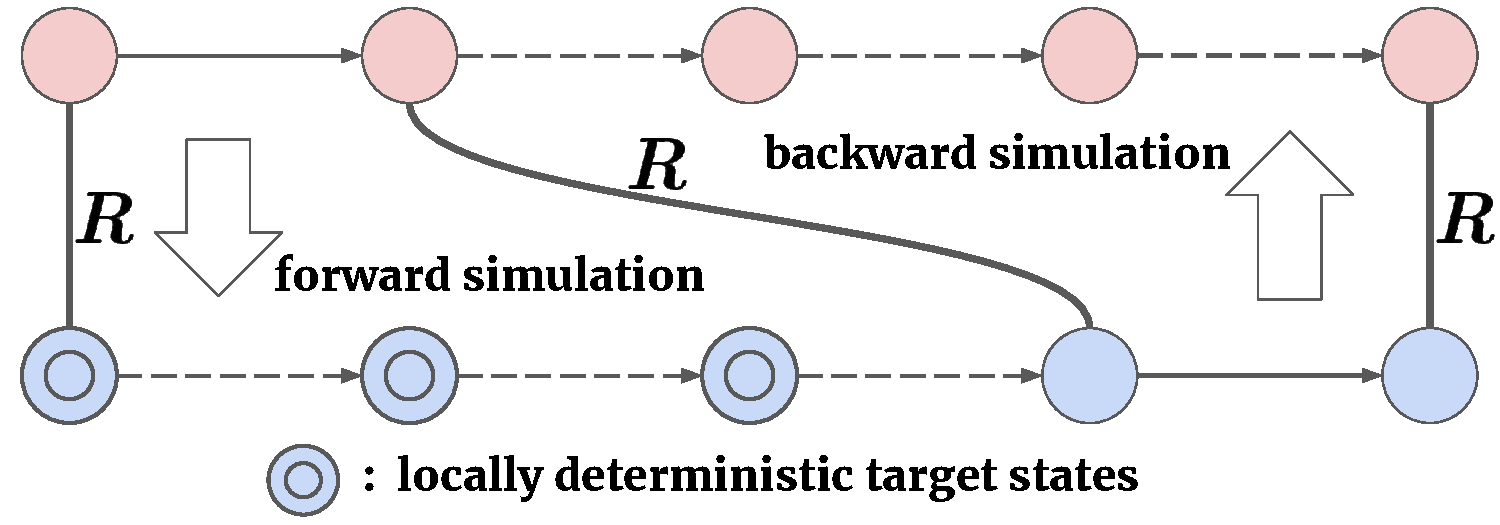
\includegraphics[width=0.7\textwidth]{images/mixed-sim-bold.pdf}
%% 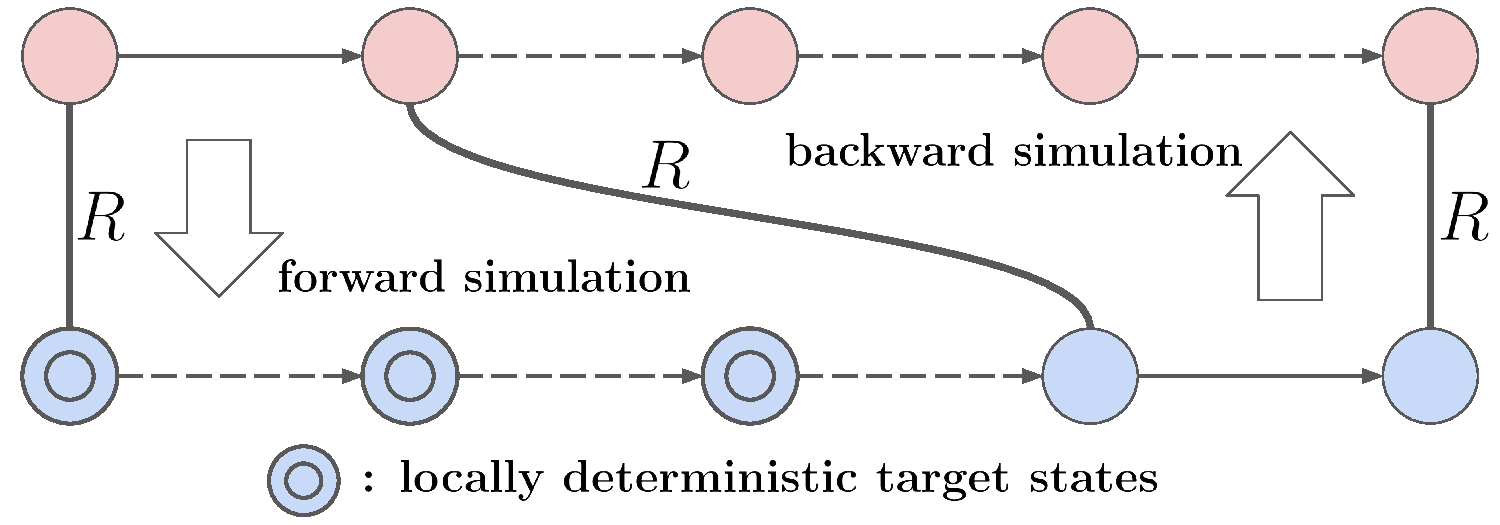
\includegraphics[width=0.7\textwidth]{images/mixed-sim.pdf}
\caption{A visualized example of mixed simulations}
\label{fig:mixedsim}
\end{figure}

%% Using mixed simulation, we verify the compositional correctness of \cc{} optimizations by
%% performing forward reasoning on deterministic target states, thereby reusing all the simulation proofs in \cc{}
%% and performing backward reasoning on nondeterministic target states which we
%% introduce in \ccm{}.
%% Furthermore, using mixed simulation, we can reduce the trusted computing base
%% of the original \cc{} by removing the assumption that external function calls are deterministic.
%% Mixed simulation is the first embodiment of the idea of exploiting determinism at the granularity of
%% machine states in the context of \cc{}, while the idea itself is first presented in
%% \cite{neis:pilsner}.

%% Specifically, \cc{}'s forward simulation actually requires a notion slightly different from
%% determinism (namely, that the source language is \emph{receptive} and the target language is
%% \emph{determinate}).  Our formalization supports both \cc{}-style forward simulation and the
%% Pilsner's one.

%%% Local Variables:
%%% mode: latex
%%% TeX-master: "main"
%%% End:
